\begin{frame}
  \frametitle{Les outils actuels}
  \begin{block}{Papi}
  \begin{itemize}
    \item Compteur hardware
    \item Basé sur l'architecture de la machine
    \item Paramètres difficillement simulables
    \end{itemize}    
  \end{block}
  \begin{block}{Cachegrind}
    \begin{itemize}
    \item Simulation d'un thread
    \item Execution séquentielle
    \item Architecture associé à la machine
    \end{itemize}
  \end{block}   
\end{frame}

\begin{frame}
  \frametitle{Projet CASSIS}
  A quels besoins répond le projet CASSIS?
  \newline
  \begin{itemize}  
  \item Rejouer une éxécution mutli-threadés
    \newline
  \item Architecture libre
    \newline
  \item Gestion des données
    \newline
  \item Modularité
  \end{itemize}  
\end{frame}




\begin{frame}
  \frametitle{Autour de CASSIS}
  \begin{figure}
    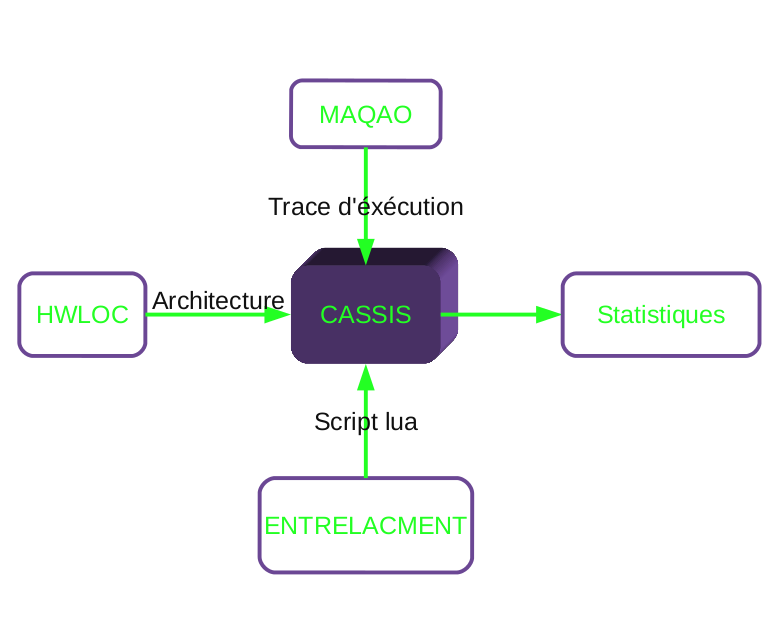
\includegraphics[scale=0.4]{images/schema_cassis.png}
  \end{figure}
\end{frame}
